% \documentclass[conference]{IEEEtran}

% \begin{document}
% \title{An Important Conference Contribution}

% \author{\IEEEauthorblockN{Author One\IEEEauthorrefmark{1},
% Author Two\IEEEauthorrefmark{2}, Author Three\IEEEauthorrefmark{3} and
% Author Four\IEEEauthorrefmark{4}}
% \IEEEauthorblockA{Department of Whatever,
% Whichever University\\
% Wherever\\
% Email: \IEEEauthorrefmark{1}author.one@add.on.net,
% \IEEEauthorrefmark{2}author.two@add.on.net,
% \IEEEauthorrefmark{3}author.three@add.on.net,
% \IEEEauthorrefmark{4}author.four@add.on.net}}
% \maketitle

% \end{document}


\documentclass[conference]{IEEEtran}
\usepackage{blindtext, graphicx}
\usepackage{fancyhdr} 
\graphicspath{ {images/} }
\fancyhf{}
\cfoot{\thepage}
\pagestyle{fancy}

% *** GRAPHICS RELATED PACKAGES ***
%
\ifCLASSINFOpdf
  % \usepackage[pdftex]{graphicx}
  % declare the path(s) where your graphic files are
  % \graphicspath{{../pdf/}{../jpeg/}}
  % and their extensions so you won't have to specify these with
  % every instance of \includegraphics
  % \DeclareGraphicsExtensions{.pdf,.jpeg,.png}
\else
  % or other class option (dvipsone, dvipdf, if not using dvips). graphicx
  % will default to the driver specified in the system graphics.cfg if no
  % driver is specified.
  % \usepackage[dvips]{graphicx}
  % declare the path(s) where your graphic files are
  % \graphicspath{{../eps/}}
  % and their extensions so you won't have to specify these with
  % every instance of \includegraphics
  % \DeclareGraphicsExtensions{.eps}
\fi






% correct bad hyphenation here
\hyphenation{op-tical net-works semi-conduc-tor}

\pagenumbering{arabic}
\begin{document}
%
% paper title
% can use linebreaks \\ within to get better formatting as desired
\title{Investigating Fault-Proneness Through Hotfix Commits: A Research in the Light of Different Programming Languages}


% author names and affiliations
% use a multiple column layout for up to three different
% affiliations
\author{\IEEEauthorblockN{Martin Lazarov\IEEEauthorrefmark{1},
Ismaa'eel Ataullah\IEEEauthorrefmark{2}, Vladyslav Kolesnyk\IEEEauthorrefmark{3},
Veselin Pavlov\IEEEauthorrefmark{4}}
\IEEEauthorblockA{Department of Computer Science,
UCL\\
Email: \IEEEauthorrefmark{1}martin.lazarov.12@ucl.ac.uk,
\IEEEauthorrefmark{2}ismaaeel.ataullah.12@ucl.ac.uk,
\IEEEauthorrefmark{3}vladyslav.kolesnyk.12@ucl.ac.uk,
\IEEEauthorrefmark{4}veselin.pavlov.15@ucl.ac.uk}}

% make the title area
\maketitle

\begin{abstract}
%\boldmath
Choosing the most suitable tools and programming languages is a very challenging task for every project manager and developer. Often the success of a software project is determined by the stability of the system after a release. In this paper, we propose analysing hotfix commits in various development areas as a means of indicating what languages tend to produce the least amount of problems after software has been published. We have focused on parsing metadata from projects hosted on SourceForge related to five specific topics (“software development”, “databases”, “security”, “games”, “front-ends”) and have performed an estimation of the amount of deployed hotfixes to compare the fault-proneness of various languages. 
\end{abstract}

\begin{IEEEkeywords}
Version Control, hotfixes, SourceForge, commits metadata.
\end{IEEEkeywords}

\section{Introduction}
Planning and resource allocation are arguably the most crucial components of any software project. Our research was motivated by the fact that very often, in the planning phase project managers neglect the importance of hotfixes – which becomes essential once a project is deployed. The most common reason for that practice is the fact that hotfixes are not constant and their presence is difficult for prediction. As a result, it is quite challenging to estimate their quantity and incorporate them into the cost of the project.  Our research attempts to provide this crucial information by correlating hotfixes with the choice of language to develop software in a specific area. As there are no clear definitions that specify what a hotfix is, according to our research and observations from the open-source projects, a hotfix can be defined as: “a corrective commit deployed within 1 day, following a project’s version update to fix critical issues in the release”.\par
We believe that the results from our research can provide insights into the average number of issues per project with a focus on different programming topics and the relevant languages used. Consequently, project managers will be able to make a more informed decision with regard to the most appropriate programming languages they could use to try to achieve a minimum number of problems in production. This will improve software engineering practices and the overall project planning activity. Furthermore, it will help optimise the allocation of resources.
The contributions of this paper are:

\begin{itemize}
  \item parameters to determine most probable hotfix commits in the repository.
  \item a quantitative analysis identifying fault-proneness of specific programming topics and the relevant distribution of faults across programming languages.
  \item an investigation into the following relationships between languages: strongly-typed vs weakly-typed, static vs dynamic and functional vs procedural to try to determine what group of languages is the most reliable.
  \item a foundation for future research in the area of identifying language-specific hotfixes.
\end{itemize}
\par
\textbf{Structure of the paper.}\\
We discuss Related Work in section 2. The next segment discusses our Solution. Following from that, an analysis of the gathered results is presented. Finally, we review our approach and findings, and examine Future Work.


\section{Related Work}
Many researchers have explored various aspects of defects in software through the use of versioning system history logs. We have also decided to follow this approach due to its openness and accessibility. This method is also very widely adopted amongst the MSR community [1]. Our investigation focused primarily on two research aspects and involved exploring existing work related to: 1) identifying hotfix commits and 2) comparison of programming languages’ stability.


\subsection{Identifying hotfix commits}
The first major problem we had to solve was identifying actual hotfix commits. Due to Boa’s limitations, we were not able to find commit history from hotfix branch. We were only capable of collecting information with regard to commits performed on the main branch. Therefore, we reviewed various papers to identify the most appropriate method of determining the type of the commit to extract only the ones related to a bug correction.\par

A large number of the reports that we studied implemented a very simple approach. They focused on the commit message as the main mechanism to try to identify whether a commit was of a corrective type [1, 4, 5]. They simply investigated if the string of text contained particular key words, such as: “bug”, “fix”, “issue”, “error”, “broke”, etc.\par

Some authors proposed a solution that involved a slightly more complex procedure including a syntactic analysis of the commit messages. Their algorithm consisted of multiple steps: 1) normalization of the data (removing non-alphanumeric characters), 2) word frequency analysis including a classification of the most common words ( e.g. “for”, “code”, “to”, “the”, etc. ) as being neutral, 3) implementing a keyword clustering algorithm to classify the commits [3].\par

Another approach to identify bug fix commits involved performing a classification based on the size of the commits [1, 3, 5]. The size of a commit can be measured based on the number of lines or the amount of files that were changed. According to these authors, large commits tend to improve code quality or add new features, while small ones are considered to be corrective - targeted at fixing bugs in the project. Some researchers proposed a further fine-grained size classification depending on the number of files changed per commit [1]. They defined the following categories: 1) tiny (1 to 5 changed files), 2) small (6 to 25 files), 3) medium (26 to 125 files), large (126 up ). The scientists further argued that most of the commits tend to be tiny (in 80\% of the cases). This implies that bug fix commits occur very often as corrective commits tend to be small ones.\par

We also looked at the time factor with regard to commits. According to some authors, issues in critical components (e.g. errors in operating system drivers, security errors) tend to be fixed relatively quickly when discovered [2]. In [3], the researchers argue that the time between changes will depend on the type of alteration. Furthermore, they hold the view that corrective changes require the least amount of time to be completed as often they have to be performed promptly regardless of the complexity of the task.\par

In terms of the time aspect, there was another paper which investigated the duration between the moment when a change is applied to a specific branch and the moment the new code was merged into the trunk [10]. However, they explored branches in general without focusing specifically on bugfix branches. Some other scientists were trying to explain people’s behaviour during commits by investigating their commit frequency distribution. As a result, they discovered that on average the time between commits was 3.206 days and half of all the contributors spent less than 13.78 hours between 50\% of their commits [11].\par

Another solution related to identifying defects in software focused on analysing commit metadata to discover design smells and predict where a break in different areas of the code may appear every time a change is performed [6]. However, they did not make their investigation language-specific as opposed to what we propose in our paper.\par

Other scientists tried to explore the logical coupling of commits as a way of identifying potential software defects. They aimed at developing a method to reduce the number of bugs in the code during the development stage so that less fix commits will be needed in the future [9].\par

A further interesting research that we found was related to the use of separate bug fix branches. According to the study performed by Phillips et al. [7], 41\% of the tested projects had incorporated an isolated bug fix branch.

\subsection{Comparison of programming languages' stability}
Throughout our investigation we discovered that there were a lot of authors that tried to utilize commit data to try to propose good engineering practices and find a way to determine code quality [8]. Furthermore, there were several papers that compared and contrasted the performance of different languages, which led to our second research topic. We explored these existing scientific studies to see what techniques authors had implemented. We also analysed the hypotheses these papers proposed to increase the scope of our project.\par

Our specific point of interest was related to different software topics and programming languages to discover how number of hotfixes per topic depend on the language developers use.\par

There were researchers that focused on the effect of programming languages on software quality [12]. The authors based performance on the rate of defect occurrences in various languages. The study was carried out on a huge dataset from GitHub (1.5 million commits). To evaluate the effect that programming languages have on software quality, the authors implemented the following strategy. First, they grouped languages according to their type, i.e. strongly vs weakly typed. They also used mathematical methods to triangulate and produce statistics for how group size, project history and number of contributors affect the number of defects. In order to achieve more representative results, they took a sample of 17 languages and extracted the top 50 projects per language. The results showed how defect-prone languages are compared to others. This was done by taking a grand mean and then comparing each language to the grand mean. Languages were then grouped, a mean was taken and then types of languages were once again compared to a grand mean - e.g. functional-strong-static languages compared to functional-dynamic-strong languages. This research focused on classifying bugs based on their type as opposed to our investigation, where we focused specifically on the distribution of hotfixes across programming languages.\par

In [13] Java and C++ were evaluated by comparing bug rates. In this case, there were two definitions for bugs - a defect and a bug itself. A defect included issues such as syntax errors, logical errors and changes in variable name. A bug itself was only defined to be a problem detected during testing or deployment. The mean number of defects and bugs, averaged over a number of projects, was compared between both languages per 1000 lines of code. The scientists also compared observed defects and bugs per hour as well as the time taken to fix defects in both languages. Productivity was also measured by analysing number of lines written per second.\par

There were researchers that used slightly different parameters to compare programming languages, these included program length, programming effort, run-time efficiency, memory consumption, and reliability [14].\par

An interesting paper that we reviewed analysed memory usage and speed of execution of three different bioinformatics methods for six distinct programming languages [15]. This was especially pertinent as bioinformatics applications have huge datasets and computational time taken is not trivial, hence optimising speed is desirable.\par

Another group of authors compared 8 different languages by conciseness, size of executables, running time, memory usage and failure proneness [16]. They argued that conciseness is an important factor as a more compact language can help write a program with fewer bugs.


\section{Solution}
Our hypothesis was motivated by research paper [12]. In it the authors compared the number of bug commits to the total number of commits across 17 languages and 850 different projects.\par

We were interested in investigating whether their findings applied when comparing number of hotfixes to total number of commits and if those conclusions were still relevant when we divided our project sources into various topics.\par

More specifically we wanted to see whether:
\begin{enumerate}
\item \textbf{Strongly-typed languages required fewer hotfixes than weakly-typed languages.}
\item \textbf{Statically-typed languages required fewer hotfixes than dynamically-typed languages.}
\item \textbf{Functional languages required fewer hotfixes than procedural ones.}
\end{enumerate}
\par
In order to evaluate our hypothesis, we developed a tool in Boa [17] that would allow us to incorporate our ideas and perform an analysis to verify them. Next, we present our reasoning and what factors we considered to accomplish our research.\par

To calculate the frequency of hotfixes for various projects and topics, we had to design a way of distinguishing a hotfix based on the commit messages. Based on the definition of a hotfix, we focused on discovering corrective commits that were submitted quickly after a new version release. In this way, we were hoping to identify problems specifically related to the version update. Therefore, we decided to divide our implementation into: detecting a \textbf{version bump commit} (i.e. a commit indicating a version increase) and identifying subsequent \textbf{bug fix commits}.\par

Unfortunately, no prior projects implemented a technique to detect version bump commits. However, from the observed data it turned out to be quite straightforward to extract this information by generating a regular expression to match strings like: “bump”, “version”, “update” in an appropriate order.\par

From our Related Work, we found projects [1, 4, 5], which distinguished bug fix commits only based on the commit messages. However, due to the similarity between commit messages for normal bug fixes and hotfix commits, and occasionally the large sequences of text, it was challenging to use the same approach. Therefore, in addition to bug fix commit detection, we applied some other parameters to ensure that it is not just a regular fix, but a hotfix. As previously discussed, we used a regular expression which examined commit messages for words associated with a corrective commit (e.g. “bug”, “fix”, “issue”, “error”, “broke”, etc.) to detect all bug fix commits. Next, we considered other possibilities that would let us detect hotfixes in a more reliable way. Some of the papers we discussed in Related Work [1, 3, 5, 11] incorporated metadata, such as: the size of changes (the number of files that were altered) and the time of the commit (how long it took for a patch to be submitted) to identify bug fixes. We considered these options for our purposes as well. Consequently, in order to increase our confidence level that the current fix commit is an actual hotfix, we introduced the following parameters to verify the emergency of the fix:
\begin{itemize}
  \item \textbf{Time} - commits have to be submitted within 1 day from the version bump commit
  \item \textbf{Look-ahead} range for commits - only n numbers of commits should be considered after version bump
\end{itemize}

\par
The size of the commit (i.e. Number of files changed ) could have been used as another parameter to determine hotfixes as our investigation discovered that corrective type of changes generally affect few files (e.g. revert new alterations or switch off a problematic feature). However, based on our results, we found examples where lots of changes were merged into one commit. Consequently, several hotfixes may be submitted as part of a single merge commit, hence affecting many files. In such case, we would fail to account for these hotfix commits because of the large number of files involved in the fix.\par

The reason why we decided to put a limit and investigate commits only within 1 day after a release was because of the nature of hotfixes. Whenever a live product contains a critical fault, it tends to be identified quickly as key functionalities stop working. Therefore, leaving bugs in production amplify the risk of the system being unusable. As a result, such hotfixes are assigned the highest priority and have to be performed rapidly even outside of the normal development process.\par

Furthermore, it is very likely that fixes performed on the first day after a new release will refer to problems occurring before the version increase (or at latest to commits submitted on that day). Therefore, we decided to focus on the Look-ahead to investigate the first n commits after a version update. We focused on the first 15 commits as anything after this point would increase the probability that a fix is related to code added after the release rather than before that. To provide more fine-grained results, we looked at the initial 5, 10 and 15 commits separately.\par

With regard to evaluating the most optimal Look-ahead value, we decided to count the number of Forward Engineering commits as well (i.e. commits that introduce new features). We did this because we were interested in identifying the largest fix commits/forward commits ratio. This would allow us to guarantee that lower number of new features were introduced into the code and consequently that some of the higher number of fixes refer to the previous version.\par

Based on our research and the experiments we ran, we managed to identify the most optimal parameters (i.e. \textbf{time}: within 1 day after a release and \textbf{look-ahead}: the first 10 commits - \textit{see Table 1 in Appendix}). Having accomplished that, we focused on selecting a dataset. We decided to analyse SourceForge 2013 because it provided categorisation of projects into programming topics (e.g. code related to: “databases”, “software development”, “security”, etc.). Unfortunately, Github did not possess such classification. We believed that being able to sort projects based on topics would produce greater insights and more useful information for developers, as they would be more interested in language efficiency for particular software development area.\par

From all the available projects, we only concentrated on the ones that had incorporated versioning (i.e. containing bump commits). Our argument was that only if there were version updates which we could detect, we would be able to perform a hotfix analysis. Therefore, we extracted all the projects that had incorporated bump commits and applied our parameters to try to recognise the hotfixes. Consequently, for each programming language we analysed the number of hotfix and bump commits so that we would be able to 
\begin{enumerate}
\item \textbf{Strongly-typed languages required fewer hotfixes than weakly-typed languages.}
\item \textbf{Statically-typed languages required fewer hotfixes than dynamically-typed languages.}
\item \textbf{Functional languages required fewer hotfixes than procedural ones.}
\end{enumerate}

\subsection{Overall performance of programming languages}
We started with investigating the overall reliability of different languages regardless of the topic they belonged to.\\
\begin{figure}
\centering
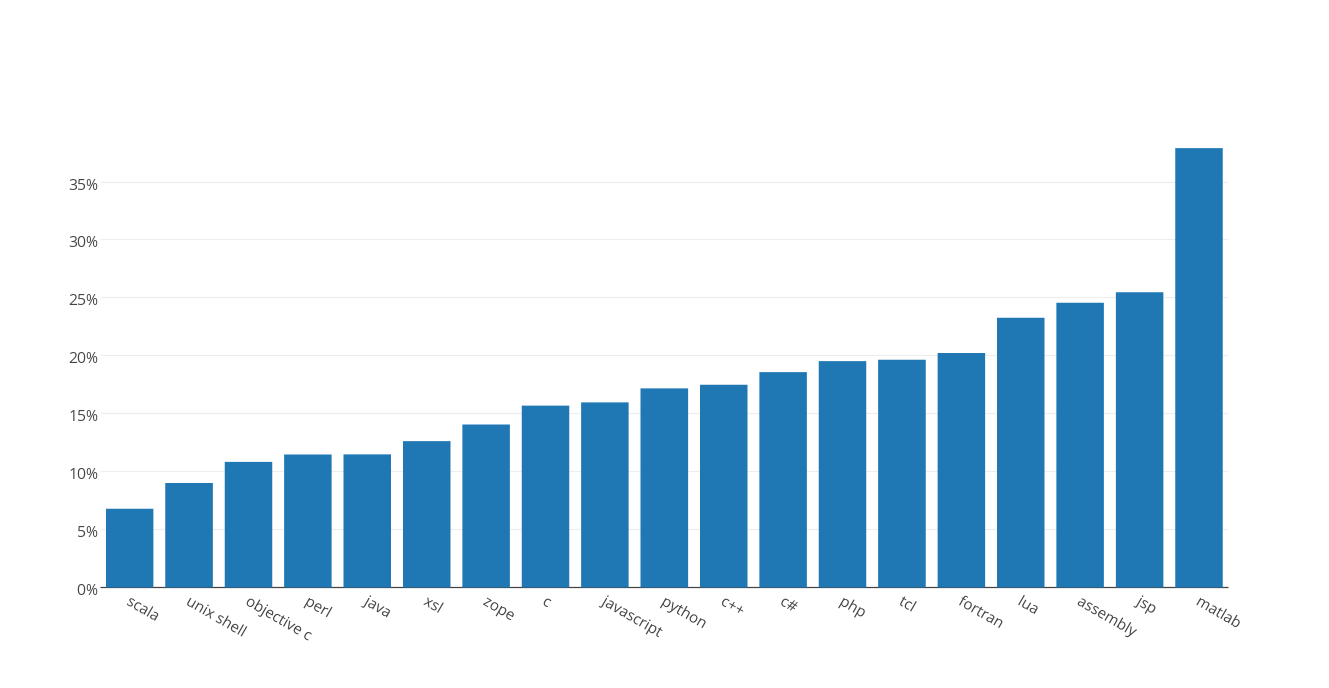
\includegraphics[width=0.75\textwidth]{Bar_chart}
\caption{Overall hotfixes per programming languages for 100 releases.}
\label{fig:my_label}
\end{figure}

\par
By performing a general analysis on all languages regardless of their topic, we compared the ratios of hotfix commit/release based on the available data. According to our results, Scala is the most reliable programming language with only 6.8 hotfixes per 100 releases ( \textit{see Table 1 in Appendix for more details}). On the other hand, Matlab is the worst performing language with 37.93 hot corrections per 100 version updates.\\

\textbf{Hypothesis 1}:\par
The strongly-typed languages we considered were: C\#, Java, Python, Scala.\par
The weakly-typed languages we identified were: C, C++, Objective C, Perl, Javascript, PHP.\par

First, Scala performs better than all weakly-typed languages. However, C\#, Java and Python do not support the hypothesis and do not outperform all weakly-typed languages. Moreover, all of them have a higher hotfix per version bump ratio than Objective C. Therefore, based on our results, we can state that it is often the case that a strongly-typed language \textbf{does not} have fewer hotfixes than a weakly-typed language and our analysis is inconclusive on this matter.\\

\textbf{Hypothesis 2}:\par
Static languages considered: C, C++, Objective C, Java, Scala.\par
Dynamic languages identified: Python, Perl, PHP, Javascript.\par

C performs better than all dynamic languages apart from Perl. 
C++ is only more reliable than PHP. In all other cases, C++ contains more hotfixes than the other dynamically-typed languages. 
Objective C is a very strong static candidate and is more reliable than all dynamic languages. Java performs slightly worse, but it still has overall dominance over the dynamically-typed languages. It has more amount of hotfixes per release only when compared with Perl. However, in the other cases, it is more efficient than all languages from the second group. Scala, as shown already is the best performer throughout all languages. Therefore, it is more reliable than all dynamic ones. From this analysis, we could say that in most of the cases, the second part of our hypothesis \textbf{is supported} by the results we obtained.\\

\textbf{Hypothesis 3}:\par
Unfortunately, from the languages that we were able to collect information about, only Scala is a member of the functional programming languages. As mentioned already Scala is the best performer amongst all evaluated languages, and as such will undoubtedly have less hotfixes than all the procedural languages (e.g. C, C++,C\#, Objective C, Java ). Thus, based purely on our results, the third part of our hypothesis agrees with the data that we collected.\par

Overall, our hypothesis agreed with the results we obtained apart from a small number of cases. However, we expect that this may be due to the different amount of releases and hotfixes identified per language. We could also conclude that Functional-Static-Strong languages are better than Procedural-Dynamic-Weak ones. Therefore, we could also argue that by using combinations of the former type of languages, developers will be able to guarantee the lowest amount of hotfixes per release. As a result, the effort needed for maintenance will be reduced and software quality will be improved.

\subsection{Topic: Databases}
We take into account reliability as we want to reach reasonable scientific conclusions based on our findings. Unfortunately, we experience limitations within the data. For example, there are languages where we have identified only 2 or 3 bump commits. Deriving results from such a small dataset is extremely unreliable and it is not likely we can reach accurate solutions with them, hence we exclude them as outliers. These languages are Zope and C\# 1.0.\par
We can see from our results that C has the lowest number of hotfix to bump commit ratio, suggesting that C is the most reliable language to program in, closely followed by Python. C++, PHP and Javascript have similar reliability according to our results but are less stable when compared to Perl or Python. Given the large number of bump commits for C++, PHP and Javascript, we can assume these results are reliable.\par
Our hypothesis had three aspects to it and we will analyse whether our results support all of them.\\

\textbf{Hypothesis 1}:\par
The strongly typed languages we consider are: Java, Python.\par
The weakly typed languages we consider are: C, C++, Perl, PHP, Javascript.\par
In this case we have a mixed series of results which suggest that this part of our hypothesis may not be entirely correct. Although Python is ranked as the second most reliable language, it is topped by C, which is a weakly-typed language. If Java had been placed third,  the hypothesis would have been better supported as we could have then treated C as an outlier. However, this is not the case. Above Java is another weakly-typed language, namely Perl. In conclusion, when considering database-specific projects, we cannot say that Strongly-typed languages required fewer hotfixes when compared to weakly-typed ones.\\

\textbf{Hypothesis 2}:\par
The statically-typed languages we consider are: C, Java, C++.\par
The dynamically-typed languages we consider are: Javascript, Python, Perl, PHP.\par

Again we have a mixed list of results. C is top and this would suggest that statically-typed languages indeed do require fewer hotfixes when compared to dynamically-typed languages. However, the other static languages, Java and C++, are in the bottom half of the table in terms of reliability. Once again, we cannot say that this part of our hypothesis is supported when comparing languages used for developing database-specific programmes.\\

\textbf{Hypothesis 3}:\par
We cannot compare this aspect of the hypothesis as no languages in this set of results are classified as Functional languages.\par
\textbf{In conclusion},no elements of our hypotheses were supported by our results. In two cases, our observations were not definitive and in the other we did not have the required results to make a comparison. We can conclude that our hypothesis is not supported when considering languages used for developing  database-related projects.

\subsection{Topic: Games}
In order to only analyse those results we deem reliable, we will exclude C\#, Javascript and Objective C on the basis that the number of bump commits analysed for them were too low.\par

We can see from our results that for programming games, Java seems to be the most reliable language to use. C is second; however, it is somewhat behind, with 24.6\% of all commits being hotfix commits. C and C++ are very similar and are only separated by 0.1\%. In last place is Python which has a hotfix rate of almost 30\% and according to our results is the least reliable language to use.\\

\textbf{Hypothesis 1}:\par
The strongly-typed languages we consider are: Java, Python.\par
The weakly-typed languages we consider are: C, C++.\par

Java is the most reliable language by far according to our results. C, C++ and Python have quite similar hotfix rates. Java is a strongly-typed language which has a definitive advantage over the others. Thus, we can say this aspect of our hypothesis is somewhat supported. It’s only partially justified because while Python, C and C++ have similar hotfix rates, Python still ranks at the bottom of our results table.\\

\textbf{Hypothesis 2}:\par

The statically-typed languages we consider are: C, Java, C++.\par
The dynamically-typed languages we consider are: Python.\par

This aspect of the hypothesis is categorically supported by our results, all statically-typed languages are ranked higher than the dynamically-typed Python in our results. We can therefore conclude that static languages required fewer hotfixes when compared to dynamic languages and hence the latter are less reliable when programming games.\\

\textbf{Hypothesis 3}:\par
We cannot compare this aspect of the hypothesis as no languages in this set of results are classed as Functional languages.\par

\textbf{In conclusion}, we can state that our overall hypothesis is somewhat supported with regard to projects labeled as Games.

\subsection{Topic: Front-ends}
Here we can see a huge difference in numbers of bump commits detected in various projects. Thus, we can argue that not many projects were observed to have a Front-end label for sufficient analysis. And many other popular Front-end languages (e.g. Javascript, C\#) were not identified.\par
Hence, after removing languages with a small number of detected projects, we ended up with \textbf{Scala} and \textbf{Java}, where the former has a slightly smaller hotfixes per bump ratio.\\

\textbf{Hypothesis 1}:\par
Both Scala and Java are considered to be strongly-typed; thus, no comparison can be made within the filtered languages. 
Regarding all the languages, we can observe that Java and Scala, overall, have more reliable statistics than weakly-typed (PHP, C, Perl), hence the hypothesis is \textbf{satisfied}.\\

\textbf{Hypothesis 2}:\par
Both Scala and Java are classified as statically-typed; therefore, no comparison can be made within the filtered languages. In terms of all the languages in the list, we can observe that most of the static ones (C++, Scala and Java) are more reliable than dynamic languages (PHP, Perl), hence the hypothesis is \textbf{satisfied}.\\

\textbf{Hypothesis 3}:\par
From the set of languages, only Scala is considered to be functional and it indeed performed better than all the others, therefore the hypothesis is \textbf{satisfied}.

\subsection{Topic: Software Development}
We filtered languages that had insignificant number of projects under the Software Development label and ended up analysing: Java, C++, Python and C languages. It turns out Java appeared to be the most stable language, where on average for 10 version updates, only 1 hotfix would be detected.\\

\textbf{Hypothesis 1}:\par
There was no enough evidence to suggest that \textbf{all} strongly-typed languages (Java, Python) performed better than the weakly-typed ones (C++, C) within the Software Development topic. For example, Python(22.22\%) has more hotfixes than C++ (19.05\%). However, the average ratio for strongly-typed languages (16.5\%) is lower than the average ratio for weakly-typed (21.63\%). Thus, we can conclude that the hypothesis is \textbf{satisfied} in general.\\

\textbf{Hypothesis 2}:\par
Not all static languages would satisfy the hypothesis, as for example, Python as a dynamic language outperforms C (defined as a statically-typed language). However, by considering the average ratio of filtered languages, we can see that static languages (Java, C++, C - 19.1\%) by far outweigh the dynamic language Python - 22.2\%.Hence, the hypothesis is \textbf{satisfied}, however \textbf{dynamic languages are not represented} well in the dataset.\\

\textbf{Hypothesis 3}:\par
No functional languages were presented in dataset. Therefore, we cannot provide any conclusive argument with regard to the third component of our hypothesis.

\subsection{Topic: Security}
Due to the low number of releases per language that we were able to identify, we cannot guarantee that the results we collected would hold in general. However, in order to be able to perform some analysis on the data and reach somewhat valid results, we decided to exclude only the outlier languages  (i.e. the ones containing the lowest number of version updates). Thus, we decided to eliminate C\# and Python from the list of evaluated languages.\par

According to our filtered data, the best performing language is C with just 1 hotfix per 20 releases on average. On the other hand, the least reliable one is C++ as it requires a hotfix for approximately every 6.5 releases.\\

\textbf{Hypothesis 1}:\par
The analysis of our results reveals that strongly-typed languages (Java) do not perform better in comparison with weakly-typed languages (C, C++, Javascript, Perl, PHP). In fact, Java only outperforms C++, but in all other cases, it requires more hotfixes than the remaining weakly-typed languages (C, Javascript, Perl, PHP). Therefore, the first part of our hypothesis does not hold for projects related to Security.\\

\textbf{Hypothesis 2}:\par
Our observations were inconclusive on whether static languages (C, C++, Java) are more reliable than dynamic ones (Javascript, Perl, PHP). Based on our results, C performed better than all dynamically-typed languages. However, Java and C++ both required more hotfixes per version update than all dynamic languages. Therefore, our analysis cannot provide a convincing argument whether static languages are more reliable than dynamic ones. As a result, the second part of our hypothesis is inconclusive on this matter.\\

\textbf{Hypothesis 3}:\par
Unfortunately, from the results that we obtained, we could not find any functional languages to compare them to procedural ones (C, C++, Java).
Consequently, regarding the languages used in Security related projects, we are not capable of deriving any conclusions about the required number of hotfixes whatsoever. Thus, there is no argument to support or disprove the third element of our hypothesis.\par
Overall, due to the insufficient number of releases in our data, we were not able to state conclusively whether our hypothesis is supported or not. Although there were examples of disproving it, we believe that having information about a larger amount of releases may actually reveal results closer to the overall observations.

\subsection{Limitations.}
There were several limitations that we encountered throughout our research:
\begin{itemize}
  \item we were able to analyse only a small part of all available projects because most of the developers did not support a versioning system, i.e. no bump commits could be identified.
  \item we could not extract hotfix branches, only the overall commits on the trunk were available and thus we used our own parameters to try to distinguish hotfix commits. Therefore, we may have introduced some false positives or failed to account for actual hotfixes.
  \item the way we detected bump commits was by writing a regular expression to match words like:  “bump”, “version”, “update” in an appropriate order. Thus, we may have excluded version updates had they been indicated differently. 
  \item most open source projects are not under the stress of releasing as opposed to commercial projects. Consequently, they do not release very often and/or do not support versioning.
  \item only one dataset was used to evaluate our hypothesis - SourceForge 2013.
\end{itemize}

\section{Conclusions and Future Work}
We have presented a research in detecting the fault-proneness of programming languages through hotfix commits - a topic that has not been investigated so far. To increase the significance of our study we performed both an overall estimation of hotfixes and a topic-specific analysis. The tool that we created was written in Boa and mined repositories from SourceForge 2013’s dataset. Our goal was to verify whether the general relationships between languages’ reliability holds with regard to hotfixes. Specifically, we investigated the following relations: strongly-typed vs weakly-typed languages, static vs dynamic and functional vs procedural. We expected that in each pair the first group of languages will be dominant. Although our overall results supported our hypothesis, on a topic-by-topic basis we were not able to verify it.\par
Therefore, we believe that some future work has to be accomplished to increase the validity of our observations. In particular, more datasets could be used, including Github (provided that projects are categorised into topics). Further improvements may be done to identify bump commits more accurately. Recently, a few commercial projects have been open-sourced and as a result, we could use them to enhance the quality of our data. In such projects, releases will have occurred more frequently and thus, there is a higher probability of identifying more hotfixes.\par
Finally, we believe that our paper provides a good foundation for future research to be done in this topic. We expect that the results we obtained will help developers and project managers improve their planning and understand what the most appropriate languages are for their specific topic.






% An example of a floating table. Note that, for IEEE style tables, the 
% \caption command should come BEFORE the table. Table text will default to
% \footnotesize as IEEE normally uses this smaller font for tables.
% The \label must come after \caption as always.
%
%\begin{table}[!t]
%% increase table row spacing, adjust to taste
%\renewcommand{\arraystretch}{1.3}
% if using array.sty, it might be a good idea to tweak the value of
% \extrarowheight as needed to properly center the text within the cells
%\caption{An Example of a Table}
%\label{table_example}
%\centering
%% Some packages, such as MDW tools, offer better commands for making tables
%% than the plain LaTeX2e tabular which is used here.
%\begin{tabular}{|c||c|}
%\hline
%One & Two\\
%\hline
%Three & Four\\
%\hline
%\end{tabular}
%\end{table}




% if have a single appendix:
%\appendix[Proof of the Zonklar Equations]
% or
%\appendix  % for no appendix heading
% do not use \section anymore after \appendix, only \section*
% is possibly needed

% use appendices with more than one appendix
% then use \section to start each appendix
% you must declare a \section before using any
% \subsection or using \label (\appendices by itself
% starts a section numbered zero.)
%



% Can use something like this to put references on a page
% by themselves when using endfloat and the captionsoff option.
\ifCLASSOPTIONcaptionsoff
  \newpage
\fi



% trigger a \newpage just before the given reference
% number - used to balance the columns on the last page
% adjust value as needed - may need to be readjusted if
% the document is modified later
%\IEEEtriggeratref{8}
% The "triggered" command can be changed if desired:
%\IEEEtriggercmd{\enlargethispage{-5in}}

% references section

% can use a bibliography generated by BibTeX as a .bbl file
% BibTeX documentation can be easily obtained at:
% http://www.ctan.org/tex-archive/biblio/bibtex/contrib/doc/
% The IEEEtran BibTeX style support page is at:
% http://www.michaelshell.org/tex/ieeetran/bibtex/
%\bibliographystyle{IEEEtran}
% argument is your BibTeX string definitions and bibliography database(s)
%\bibliography{IEEEabrv,../bib/paper}
%
% <OR> manually copy in the resultant .bbl file
% set second argument of \begin to the number of references
% (used to reserve space for the reference number labels box)
\begin{thebibliography}{1}
\bibitem{}
Hattori, L.P.; Lanza, M., \emph{"On the nature of commits"} in Automated Software Engineering - Workshops, 2008. ASE Workshops 2008. 23rd IEEE/ACM International Conference on , vol., no., pp.63-71, 15-16 Sept. 2008
\bibitem{}
Livshits,B.; Zimmerman,T.; \emph{"DynaMine: Finding Common Error Patterns by Mining Software Revision Histories"} in Proceedings of the 10th European software engineering conference held jointly with 13th ACM SIGSOFT international symposium on Foundations of software engineering, pp.296-305
\bibitem{}
Mockus, A.; Votta, L.G., \emph{"Identifying reasons for software changes using historic databases"} in Software Maintenance, 2000. Proceedings. International Conference on , vol., no., pp.120-130, 2000
\bibitem{}
Ratzinger,J.; Sigmund,T.; Gall,H.; \emph{"On the Relation of Refactoring and Software Defects"} in MSR '08, Proceedings of the 2008 international working conference on Mining software repositories, pp. 35-38
\bibitem{}
Hindle,A.; German,D.; Holt,R.; \emph{"What do large commits tell us?: a taxonomical study of large commits"} in MSR '08, Proceedings of the 2008 international working conference on Mining software repositories, pp.99-108
\bibitem{}
Oliva,G.; Steinmacher,I.; Wiese,I.; Aurelio,M.; \emph{"What Can Commit Metadata Tell Us About Design Degradation?"} in IWPSE 2013, Proceedings of the 2013 International Workshop on Principles of Software Evolution, pp.18-27
\bibitem{}
Phillips,S.; Sillito,J.; Walker,R.; \emph{"Branching and merging: an investigation into current version control practices"} in CHASE '11 Proceedings of the 4th International Workshop on Cooperative and Human Aspects of Software Engineering, pp.9-15
\bibitem{}
Agrawal, K.; Amreen, S.; Mockus, A., \emph{"Commit Quality in Five High Performance Computing Projects"} in Software Engineering for High Performance Computing in Science (SE4HPCS), 2015 IEEE/ACM 1st International Workshop on , vol., no., pp.24-29, 18-18 May 2015
\bibitem{}
Steff, M.; Russo, B., \emph{"Co-evolution of logical couplings and commits for defect estimation"} in Mining Software Repositories (MSR), 2012 9th IEEE Working Conference on , vol., no., pp.213-216, 2-3 June 2012
\bibitem{}
Williams,C.; Spacco,J.; \emph{"Branching and Merging in the Repository"} in MSR '08, Proceedings of the 2008 international working conference on Mining software repositories, pp.19-22
\bibitem{}
Kolassa,C.; Riehle,D.; Salim,M.; \emph{"The Empirical Commit Frequency Distribution of Open Source Projects"} in WikiSym '13, Proceedings of the 9th International Symposium on Open Collaboration, Article No.18
\bibitem{}
Ray,B.; Posnett,D.; Filkov,V.; Devanbu,P;  \emph{A Large Scale Study of Programming Languages and Code Quality"} in Github;  FSE 2014, Proceedings of the 22nd ACM SIGSOFT International Symposium on Foundations of Software Engineering, pp.155-165
\bibitem{}
Phipps,G; \emph{"Comparing Observed Bug and Productivity Rates for Java and C++" } in Software—Practice \& Experience; vol.29, issue 4, pp.345-358, April 10, 1999 
\bibitem{}
Prechelt, L., \emph{"An empirical comparison of seven programming languages"} in Computer , vol.33, no.10, pp.23-29, Oct 2000
\bibitem{}
Fourment,M.; Gillings,M.; \emph{"A comparison of common programming languages used in bioinformatics"} in BMC Bioinformatics Feb 2008
\bibitem{}
Furia,C.; Nanz,S.; \emph{"A Comparative Study of Programming Languages in Rosetta Code"} in ICSE '15, Proceedings of the 37th International Conference on Software Engineering, vol.1, pp.778-788
\bibitem{}
Iowa State University of Science and Technology,  \emph{"Boa - Mining Ultra-Large-Scale Software Repositories"}, http://boa.cs.iastate.edu/


\end{thebibliography}

% biography section
% 
% If you have an EPS/PDF photo (graphicx package needed) extra braces are
% needed around the contents of the optional argument to biography to prevent
% the LaTeX parser from getting confused when it sees the complicated
% \includegraphics command within an optional argument. (You could create
% your own custom macro containing the \includegraphics command to make things
% simpler here.)
%\begin{biography}[{\includegraphics[width=1in,height=1.25in,clip,keepaspectratio]{mshell}}]{Michael Shell}
% or if you just want to reserve a space for a photo:

% You can push biographies down or up by placing
% a \vfill before or after them. The appropriate
% use of \vfill depends on what kind of text is
% on the last page and whether or not the columns
% are being equalized.

%\vfill

% Can be used to pull up biographies so that the bottom of the last one
% is flush with the other column.
%\enlargethispage{-5in}




% that's all folks
\end{document}


